% Template mimicking the Linnaeus University powerpoint template
% https://lnu.se/en/medarbetare/support-and-service/communications-and-marketing/Designmanual/templates/

\documentclass[english,9pt]{Linnaeus}
\usepackage{babel}
\usepackage{braket}
\usepackage{array,booktabs,times,mathptmx}
\usepackage{tikz}
\usepackage{amsfonts} % Para \mathbb
\usepackage{quantikz}


\usetikzlibrary{shapes.symbols}
\usetikzlibrary{calc,arrows.meta}

\newcommand{\drawparal}[7]{ % pos_x, pos_y, v_x, v_y, v_z, label, id
  \begin{scope}[shift={(#1,#2)}]
    \coordinate (O) at (0,0);
  \coordinate (A) at #3; % x-vector
    \coordinate (B) at #4; % y-vector
    \coordinate (C) at #5; % z-vector
    \coordinate (Vab) at ($ (A) + (B) $);
  \coordinate (Vac) at ($ (A) + (C) $);
  \coordinate (Vbc) at ($ (B) + (C) $);
  \coordinate (Vabc) at ($ (A) + (B) + (C) $);
  % Outer contours
    \draw[line width=0.8pt, contour] (A) -- (Vab) -- (B);
  \draw[line width=0.8pt, contour] (B) -- (Vbc) -- (C);
  \draw[line width=0.8pt, contour] (C) -- (Vac) -- (A);
  \draw[line width=0.8pt, contour] (Vab) -- (Vabc);
  \draw[line width=0.8pt, contour] (Vbc) -- (Vabc);
  \draw[line width=0.8pt, contour] (Vac) -- (Vabc);
  % Inner axes with arrows
    \draw[eje] (O) -- (A);
  \draw[eje] (O) -- (B);
  \draw[eje] (O) -- (C);
  % Label positioned in the middle of the front-facing face
    \node[anchor=center, inner sep=1.5pt] at ($ 0.5*#3 + 0.5*#4 $) {#6};

  % Define target coordinate for connection lines (origin of each para, global scope)
    \global\coordinate (#7_orig) at (0,0);
  \end{scope}
}

% Uncomment below for specific features

% If you want to use bibtex uncomment the lines below
%\usepackage{natbib}
%    \bibpunct{(}{)}{;}{a}{}{,}
%    \renewcommand{\bibfont}{\footnotesize}        
%    \newcommand{\newblock}{.}

% If you figures are in another folder
%\graphicspath{{./Figures/}}

% To reset the font in all tables
%\let\oldtabular\tabular 
%\renewcommand{\tabular}{\tiny\oldtabular} 

\author[S1e7J]{\textbf{Sergio Montoya Ramírez}}
\institute{s.montoyar2@uniandes.edu.co}
\title{\LARGE \textbf{Quantum Error Correction Code}}
\date{}


\begin{document}

\begin{frame}[plain]
\titlepage
\end{frame}

\setbeamercolor{background canvas}{bg=white}


\begin{frame}[allowframebreaks]
\frametitle{En un computador solo tenemos bits (o qbits). Todo lo demás son códigos}

\begin{columns}[c] % La opción [c] centra el contenido verticalmente. Puedes usar [t] para alinearlo arriba.

% --- COLUMNA IZQUIERDA: GRÁFICO TIKZ ---
\begin{column}{0.5\textwidth}
\centering
% Ajustamos el tamaño del gráfico para que no se salga de la columna
\resizebox{\linewidth}{!}{%
  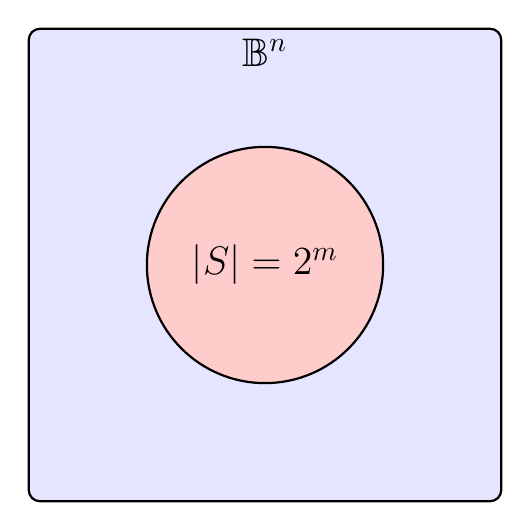
\begin{tikzpicture}
  % Definimos los estilos para los círculos
    \tikzstyle{outercircle} = [draw, thick, fill=blue!10, text centered, rounded corners, minimum width=6cm, minimum height=6cm];
  \tikzstyle{innercircle} = [draw, thick, fill=red!20, text centered, circle, minimum width=3cm];

  % Dibujamos el círculo exterior (\mathbb{B}^n)
    \node [outercircle] (Bn) at (0,0) {};
  % Etiqueta para el círculo exterior
    \node at (0, 2.7) {\Large \(\mathbb{B}^n\)};

  % Dibujamos el círculo interior (el subconjunto)
    \node [innercircle] (subset) at (0,0) {};
  % Etiqueta para la cardinalidad del subconjunto
    \node at (0, 0) {\Large \(|S| = 2^m\)};
  \end{tikzpicture}%
}
\end{column}

% --- COLUMNA DERECHA: TEXTO ---
\begin{column}{0.5\textwidth}
Un código $(n, m)$ es simplemente un subconjunto de $\mathbb{B}^n$ con $2^m$ elementos. Estos elementos pueden representar otras cosas. Por ejemplo:
\begin{enumerate}
\item Números flotantes.
\item Letras.
\item Instrucciones.
\end{enumerate}
\end{column}

\end{columns}

\end{frame}

\begin{frame}[allowframebreaks]
\frametitle{Cuando un código es cuántico, es un subespacio completo}

\begin{columns}[c]
\begin{column}{0.5\textwidth}
  \centering
% \resizebox ajusta el contenido al ancho de la línea actual (\linewidth)
  \resizebox{\linewidth}{!}{%
    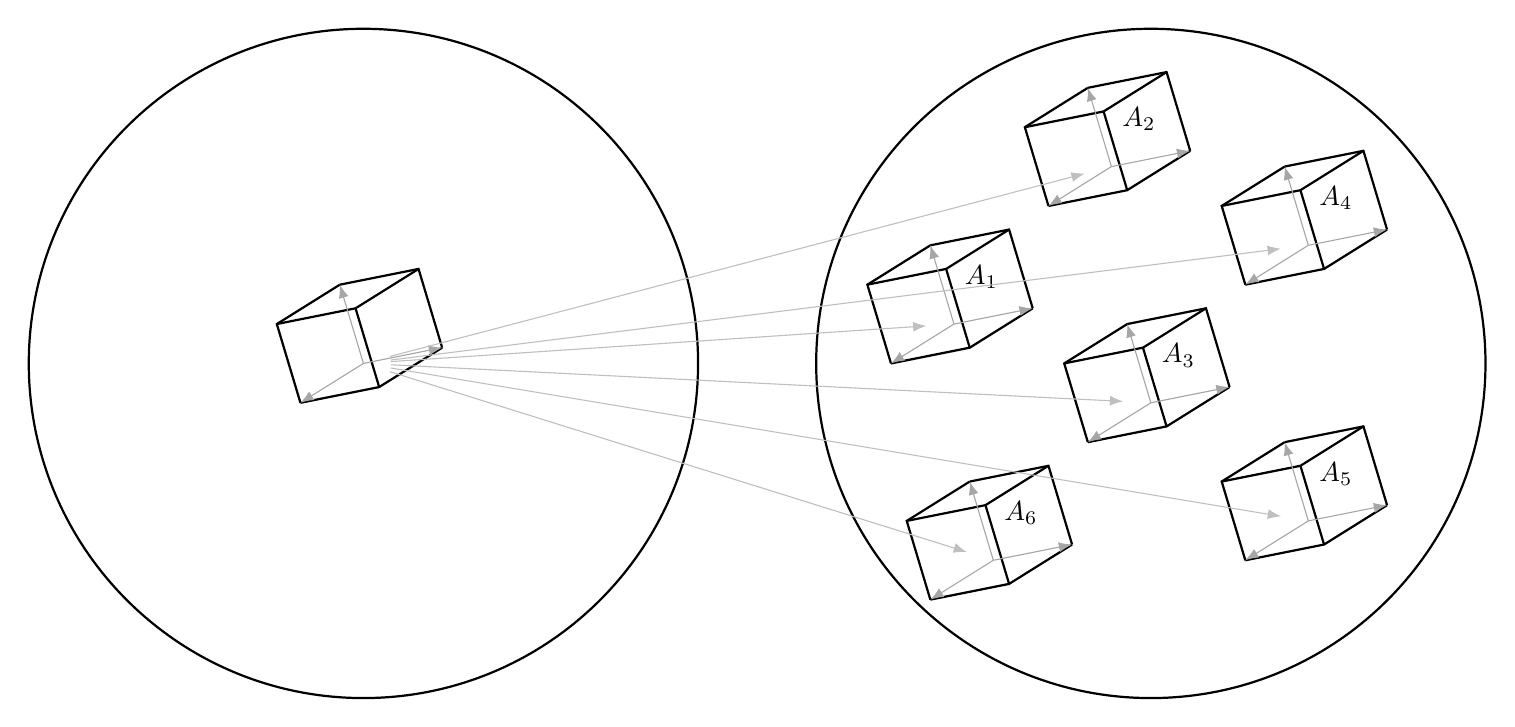
\begin{tikzpicture}[>=Latex] % Better arrows for connection lines

      % Style for inner axes and vectors
      \tikzset{eje/.style={gray!70, thin, ->}}

    % Define colors for clarity
      \colorlet{contour}{black}
    \colorlet{inner}{gray!70}
    \colorlet{connection}{gray!50}

    % Two large container circles
      \node [draw, circle, minimum size=8.5cm, line width=0.8pt] (c1) at (0,0) {};
    \node [draw, circle, minimum size=8.5cm, line width=0.8pt] (c2) at (10,0) {};

    % Draw the central cube in the first circle
      \begin{scope}[shift={(c1.center)}]
      \coordinate (o_c) at (0,0);
    \coordinate (x_c) at (1, 0.2);
    \coordinate (y_c) at (-0.3, 1);
    \coordinate (z_c) at (-0.8, -0.5);

    % Outer contours with thicker lines
      \coordinate (xy_c) at ($ (x_c) + (y_c) $);
    \coordinate (xz_c) at ($ (x_c) + (z_c) $);
    \coordinate (yz_c) at ($ (y_c) + (z_c) $);
    \coordinate (xyz_c) at ($ (x_c) + (y_c) + (z_c) $);
    \draw[line width=0.8pt, contour] (x_c) -- (xy_c) -- (y_c);
    \draw[line width=0.8pt, contour] (y_c) -- (yz_c) -- (z_c);
    \draw[line width=0.8pt, contour] (z_c) -- (xz_c) -- (x_c);
    \draw[line width=0.8pt, contour] (xy_c) -- (xyz_c);
    \draw[line width=0.8pt, contour] (yz_c) -- (xyz_c);
    \draw[line width=0.8pt, contour] (xz_c) -- (xyz_c);

    % Inner axes with arrows, drawn after contours to be visible
      \draw[eje] (o_c) -- (x_c);
    \draw[eje] (o_c) -- (y_c);
    \draw[eje] (o_c) -- (z_c);
    \end{scope}

    % Draw parallelepipeds in the second circle
      % % A1: left side, vertically oriented -> Now a uniform cube
      \drawparal{7.5}{0.5}{(1,0.2)}{(-0.3,1)}{(-0.8,-0.5)}{$A_1$}{A1}

    % A2: upper-center, tall -> Now a uniform cube
      \drawparal{9.5}{2.5}{(1,0.2)}{(-0.3,1)}{(-0.8,-0.5)}{$A_2$}{A2}

    % A3: center, wide and regular -> Now a uniform cube
      \drawparal{10}{-0.5}{(1,0.2)}{(-0.3,1)}{(-0.8,-0.5)}{$A_3$}{A3}

    % A4: upper-right, flat -> Now a uniform cube
      \drawparal{12}{1.5}{(1,0.2)}{(-0.3,1)}{(-0.8,-0.5)}{$A_4$}{A4}

    % A5: lower-right, flat -> Now a uniform cube
      \drawparal{12}{-2}{(1,0.2)}{(-0.3,1)}{(-0.8,-0.5)}{$A_5$}{A5}

    % A6: lower-left, wide -> Now a uniform cube
      \drawparal{8}{-2.5}{(1,0.2)}{(-0.3,1)}{(-0.8,-0.5)}{$A_6$}{A6}
    % Connection lines from circle 1 center to circle 2 parallelepipeds
      \coordinate (orig) at (c1.center);

    % Draw connection lines with light grey and small arrow tips
      \draw [connection, thin, ->, shorten >=10pt, shorten <=10pt] (orig) -- (A1_orig);
    \draw [connection, thin, ->, shorten >=10pt, shorten <=10pt] (orig) -- (A2_orig);
    \draw [connection, thin, ->, shorten >=10pt, shorten <=10pt] (orig) -- (A3_orig);
    \draw [connection, thin, ->, shorten >=10pt, shorten <=10pt] (orig) -- (A4_orig);
    \draw [connection, thin, ->, shorten >=10pt, shorten <=10pt] (orig) -- (A5_orig);
    \draw [connection, thin, ->, shorten >=10pt, shorten <=10pt] (orig) -- (A6_orig);

    \end{tikzpicture}%
  }
\end{column}

% --- COLUMNA DERECHA: TEXTO EXPLICATIVO ---
\begin{column}{0.5\textwidth}
Un código cuántico es un subespacio con las mismas características que antes. Sin embargo, para tener mejor control sobre él (y porque lo vamos a usar así al corregir errores) tiene que cumplir las características de:
\begin{enumerate}
\item Ser ortogonales.
\item Ser distinguibles.
\item No estar deformados.
\end{enumerate}
\end{column}
\end{columns}
\end{frame}

\begin{frame}[allowframebreaks]
\frametitle{Un error es, esencialmente, una operación que tú no controlas}
Un error es:
\begin{align}
\begin{split}
(\alpha_0\ket{0} + \alpha_1\ket{1})\ket{E} \;\to\; &\alpha_0\beta_1 \ket{0}\ket{E_1} + \alpha_0\beta_2 \ket{1}\ket{E_2}\\
    &+ \alpha_1\beta_3 \ket{0}\ket{E_3} + \alpha_1\beta_4 \ket{1}\ket{E_4}
    \end{split}
    \end{align}

    Dado que $\left\{I, X, Z, ZX\right\}$ es una base, lo podemos resumir como:

    \begin{align}
    \begin{split}
    &\frac{1}{2} \left(I\ket{\psi}\left(\beta_1 \ket{E_1} + \beta_3 \ket{E_3}\right)\right.
        + Z\ket{\psi}\left(\beta_1 \ket{E_1} - \beta_3 \ket{E_3}\right)\\
        & + X\ket{\psi}\left(\beta_2 \ket{E_2} + \beta_4 \ket{E_4}\right)
        \left. + ZX\ket{\psi}\left(\beta_2 \ket{E_2} - \beta_3 \ket{E_4}\right)\right)\\
      \end{split}
      \end{align}
      \end{frame}

      \begin{frame}[allowframebreaks]
      \frametitle{Un código corrige un error cuando existe un proceso de recuperación}
      Sea $\mathcal{E}$ un error. Se dice que un código $C$ lo corrige si existe una operación que preserva la traza, $\mathcal{R}$, tal que:
      \begin{align}
      \forall \rho \in C \implies (\mathcal{R} \circ \mathcal{E}) \rho \propto \rho
      \end{align}

      Note que existen errores que no preservan la traza y, por tanto, al corregirlos no se obtiene el mismo estado, sino uno proporcional a este.
      \end{frame}

      \begin{frame}[allowframebreaks]
      \frametitle{Demostrar que un código corrige un error no es trivial}
      Sea $C$ un código cuántico con un proyector $P$ y $\mathcal{E}$ un operador con elementos $\left\{ E_i \right\}$. El código $C$ corrige $\mathcal{E}$ si y solamente si:
      \begin{align}
      PE^\dagger_iE_jP &= \alpha_{ij}P
      \end{align}

      Para alguna matriz hermítica $\alpha$.
      \end{frame}

      \begin{frame}[allowframebreaks]
      \frametitle{Un ejemplo simple: El código de repetición permite corregir ante bitflips de un solo qbit}

      \begin{columns}[c]
      \begin{column}{0.5\textwidth}
  \centering
% \resizebox ajusta el contenido al ancho de la línea actual (\linewidth)
  \resizebox{\linewidth}{!}{%
    \begin{quantikz}
    \lstick{$\ket{\psi}$} & \qw & \qw & \ctrl{1} & \ctrl{2} & \qw & & \lstick{$\ket{\psi}$} \\
      && \lstick{$\ket{0}$} & \targ{} & \qw & \qw & & \lstick{$\ket{\psi}$} \\
      && \lstick{$\ket{0}$} & \qw & \targ{} & \qw &  & \lstick{$\ket{\psi}$} \\
      \end{quantikz}
  }
\end{column}

% --- COLUMNA DERECHA: TEXTO EXPLICATIVO ---
\begin{column}{0.5\textwidth}
Para caracterizar este código podemos decir:
\begin{itemize}
\item \textbf{Error:} $\ket{\psi}\ket{E} \;\to\; \beta_1 \ket{\psi}\ket{E_1} + \beta_2 X\ket{\psi}\ket{E_2}$
\item \textbf{Proyector:} $P = \ket{000}\bra{000} + \ket{111}\bra{111}$
\item \textbf{Recuperación:} Se divide en dos etapas:
\begin{enumerate}
\item Identificación del error ($Z_1Z_2$ y $Z_2Z_3$).
\item Corrección aplicando la operación inversa.
\end{enumerate}
\end{itemize}
\end{column}
\end{columns}
\end{frame}

\begin{frame}[allowframebreaks]
\frametitle{Los códigos de corrección de errores, bien aplicados, permiten mejorar la fidelidad}
Recapitulando:
\begin{itemize}
\item Los códigos son esenciales para la computación en general, pues permiten representar información.
\item Un error es simplemente un operador lineal, solo que no te obedece.
\item Un código corrige un error si existe un proceso de verificación.
\item Demostrar que un código corrige un error, en general, no es trivial.
\end{itemize}
\end{frame}

\begin{frame}
\frametitle{Referencias}
\begin{itemize}
\item Kitaev, A. Yu., Shen, A., y Vyalyj, M. N. (2002). \textit{Classical and Quantum Computation}. Graduate Studies in Mathematics (Vol. 47). American Mathematical Society.

\item Nielsen, M. A., y Chuang, I. L. (2010). \textit{Quantum Computation and Quantum Information} (10th Anniversary Edition). Cambridge University Press. (BnF ISBN)

  \item Kaye, P., Laflamme, R., y Mosca, M. (2007). \textit{An Introduction to Quantum Computing}. Oxford University Press.
  \item Gottesman, D. (1997). \textit{Stabilizer Codes and Quantum Error Correction} (Tesis doctoral). California Institute of Technology. \texttt{doi:10.48550/arXiv.quant-ph/9705052}
  \end{itemize}
  \end{frame}

  \begin{frame}
  \frametitle{Verificación de errores como suma de otros Pauli}
  \begin{align*}
  &\frac{1}{2} \left(\left(\alpha_0 \ket{0} + \alpha_1 \ket{1}\right)\left(\beta_1 \ket{E_1} + \beta_3 \ket{E_3}\right)\right.\\
      & + \left(\alpha_0 \ket{0} - \alpha_1 \ket{1}\right)\left(\beta_1 \ket{E_1} - \beta_3 \ket{E_3}\right)\\
      & + \left(\alpha_0 \ket{1} + \alpha_1 \ket{0}\right)\left(\beta_2 \ket{E_2} + \beta_4 \ket{E_4}\right)\\
      &\left. + \left(\alpha_0 \ket{1} - \alpha_1 \ket{0}\right)\left(\beta_2 \ket{E_2} - \beta_3 \ket{E_4}\right)\right)\\
  =&\frac{1}{2} \left(I\ket{\psi}\left(\beta_1 \ket{E_1} + \beta_3 \ket{E_3}\right)\right.\\
      & + Z\ket{\psi}\left(\beta_1 \ket{E_1} - \beta_3 \ket{E_3}\right)\\
      & + X\ket{\psi}\left(\beta_2 \ket{E_2} + \beta_4 \ket{E_4}\right)\\
      &\left. + ZX\ket{\psi}\left(\beta_2 \ket{E_2} - \beta_3 \ket{E_4}\right)\right)
  \end{align*}
  \end{frame}
  % If you want to put references uncomment the lines below and the 
  %\begin{frame}[t,allowframebreaks]
  %    \frametitle{References}
  %    \bibliographystyle{newapa}
  %\bibliography{YourBib}
  %\end{frame}

  \end{document}
